\documentclass[12pt]{article}


%%% NOTE: the following code puts the document in
%   Times New Roman. If you want to keep it, please
%   switch your compiler to XeTeX.
%   If you are on Overleaf, see:
%   https://www.overleaf.com/learn/how-to/Changing_compiler

\usepackage{fontspec}
% Gyre Termes is TeX's copy of Times New Roman
% We don't use Times New Roman (also available)
% as it doesn't support script fonts
\setmainfont{TeX Gyre Termes}

%%%%%%%%%%%%%%%%%%%%%%%%%%%%%%%%%%%%%%%%%%%%%%%%%%%%%%%%%%%%%%%%%%%%%
%                 Copyright Howard Beck @ 2024                      %
%                                                                   %
% Made for the Association of Student Activities (ASA) at the       %
% Massachusetts Institute of Technology (MIT).                      %
%                                                                   %
% Free for use by the ASA, ASA-recognized clubs, and                %
% collections of students at MIT trying to become an ASA-recognized %
% club (ASA Organizations).                                         %
%                                                                   %
% This software may not be published or distributed except by the   %
% copyright holder or by the executive board of the ASA.            %
%                                                                   %
% Further, do not sublicense and/or sell copies of the software,    %
% and do not employ it for commercial use.                          %
%                                                                   %
% Permission is granted to ASA organizations to freely modify       %
% any part of this code for their own use, as long as the copyright %
% notice here is kept in tact, and under the previous conditions.   %
%                                                                   %
% Permission is also granted to the executive board ASA to          %
% distribute modified copies of this code (subject to the above     %
% restrictions), that may contain different copyrights, so long as  %
% the following is included:                                        %
%    Based on code written by Howard Beck, MIT Class of 2025        %
%                                                                   %
%%%%%%%%%%%%%%%%%%%%%%%%%%%%%%%%%%%%%%%%%%%%%%%%%%%%%%%%%%%%%%%%%%%%%

\usepackage[margin=1in]{geometry}
% fooders, headers
\usepackage{fancyhdr}
% reference for last page
\usepackage{lastpage}
% coloring text
\usepackage{xcolor}
% clickable references
\usepackage[destlabel=true]{hyperref}
% don't hyphenate text
\usepackage[none]{hyphenat}
% commands for changing section commands
\usepackage{titlesec}
\usepackage{setspace}
% specifications for enums and items
\usepackage[shortlabels]{enumitem}
% commands for changing table of contents
\usepackage[titles]{tocloft}

%% command specifications
% command parser
\usepackage{xparse}
% \xspace after commands
\usepackage{xspace}
% for loops
\usepackage{forloop}
% if and then
\usepackage{ifthen}
% various tools for commands
\usepackage{etoolbox}

%% importing other files (used for *-sections.aux referencing)
\usepackage{import}




\makeatletter

%%% Configuration variables
\@ifundefined{groupname}
{
    \PackageError{commands}{%
        Please specify groupname BEFORE importing commands.tex. For example, use:\MessageBreak
        \def\protect\groupname{[GROUP NAME HERE]}\MessageBreak
        \protect%%%%%%%%%%%%%%%%%%%%%%%%%%%%%%%%%%%%%%%%%%%%%%%%%%%%%%%%%%%%%%%%%%%%%
%                 Copyright Howard Beck @ 2024                      %
%                                                                   %
% Made for the Association of Student Activities (ASA) at the       %
% Massachusetts Institute of Technology (MIT).                      %
%                                                                   %
% Free for use by the ASA, ASA-recognized clubs, and                %
% collections of students at MIT trying to become an ASA-recognized %
% club (ASA Organizations).                                         %
%                                                                   %
% This software may not be published or distributed except by the   %
% copyright holder or by the executive board of the ASA.            %
%                                                                   %
% Further, do not sublicense and/or sell copies of the software,    %
% and do not employ it for commercial use.                          %
%                                                                   %
% Permission is granted to ASA organizations to freely modify       %
% any part of this code for their own use, as long as the copyright %
% notice here is kept in tact, and under the previous conditions.   %
%                                                                   %
% Permission is also granted to the executive board ASA to          %
% distribute modified copies of this code (subject to the above     %
% restrictions), that may contain different copyrights, so long as  %
% the following is included:                                        %
%    Based on code written by Howard Beck, MIT Class of 2025        %
%                                                                   %
%%%%%%%%%%%%%%%%%%%%%%%%%%%%%%%%%%%%%%%%%%%%%%%%%%%%%%%%%%%%%%%%%%%%%

\usepackage[margin=1in]{geometry}
% fooders, headers
\usepackage{fancyhdr}
% reference for last page
\usepackage{lastpage}
% coloring text
\usepackage{xcolor}
% clickable references
\usepackage[destlabel=true]{hyperref}
% don't hyphenate text
\usepackage[none]{hyphenat}
% commands for changing section commands
\usepackage{titlesec}
\usepackage{setspace}
% specifications for enums and items
\usepackage[shortlabels]{enumitem}
% commands for changing table of contents
\usepackage[titles]{tocloft}

%% command specifications
% command parser
\usepackage{xparse}
% \xspace after commands
\usepackage{xspace}
% for loops
\usepackage{forloop}
% if and then
\usepackage{ifthen}
% various tools for commands
\usepackage{etoolbox}

%% importing other files (used for *-sections.aux referencing)
\usepackage{import}




\makeatletter

%%% Configuration variables
\@ifundefined{groupname}
{
    \PackageError{commands}{%
        Please specify groupname BEFORE importing commands.tex. For example, use:\MessageBreak
        \def\protect\groupname{[GROUP NAME HERE]}\MessageBreak
        \protect%%%%%%%%%%%%%%%%%%%%%%%%%%%%%%%%%%%%%%%%%%%%%%%%%%%%%%%%%%%%%%%%%%%%%
%                 Copyright Howard Beck @ 2024                      %
%                                                                   %
% Made for the Association of Student Activities (ASA) at the       %
% Massachusetts Institute of Technology (MIT).                      %
%                                                                   %
% Free for use by the ASA, ASA-recognized clubs, and                %
% collections of students at MIT trying to become an ASA-recognized %
% club (ASA Organizations).                                         %
%                                                                   %
% This software may not be published or distributed except by the   %
% copyright holder or by the executive board of the ASA.            %
%                                                                   %
% Further, do not sublicense and/or sell copies of the software,    %
% and do not employ it for commercial use.                          %
%                                                                   %
% Permission is granted to ASA organizations to freely modify       %
% any part of this code for their own use, as long as the copyright %
% notice here is kept in tact, and under the previous conditions.   %
%                                                                   %
% Permission is also granted to the executive board ASA to          %
% distribute modified copies of this code (subject to the above     %
% restrictions), that may contain different copyrights, so long as  %
% the following is included:                                        %
%    Based on code written by Howard Beck, MIT Class of 2025        %
%                                                                   %
%%%%%%%%%%%%%%%%%%%%%%%%%%%%%%%%%%%%%%%%%%%%%%%%%%%%%%%%%%%%%%%%%%%%%

\usepackage[margin=1in]{geometry}
% fooders, headers
\usepackage{fancyhdr}
% reference for last page
\usepackage{lastpage}
% coloring text
\usepackage{xcolor}
% clickable references
\usepackage[destlabel=true]{hyperref}
% don't hyphenate text
\usepackage[none]{hyphenat}
% commands for changing section commands
\usepackage{titlesec}
\usepackage{setspace}
% specifications for enums and items
\usepackage[shortlabels]{enumitem}
% commands for changing table of contents
\usepackage[titles]{tocloft}

%% command specifications
% command parser
\usepackage{xparse}
% \xspace after commands
\usepackage{xspace}
% for loops
\usepackage{forloop}
% if and then
\usepackage{ifthen}
% various tools for commands
\usepackage{etoolbox}

%% importing other files (used for *-sections.aux referencing)
\usepackage{import}




\makeatletter

%%% Configuration variables
\@ifundefined{groupname}
{
    \PackageError{commands}{%
        Please specify groupname BEFORE importing commands.tex. For example, use:\MessageBreak
        \def\protect\groupname{[GROUP NAME HERE]}\MessageBreak
        \protect\input{commands.tex}}{}
    \def\groupname{[GROUP NAME HERE]}
}
{}
\let\@oldgroupname\groupname
\def\groupname{\@oldgroupname\xspace}

\@ifundefined{doctype}
{
    \def\doctype{Constitution}
}
{}


%%% geometry
\setlength{\headheight}{15pt}
% no paragraph indentation
\setlength{\parindent}{0cm}
% line spacing
\linespread{1.25}
\setlength{\cftbeforesecskip}{0pt}
% get rid of most \hbox errors
\tolerance=1
\emergencystretch=\maxdimen
\hyphenpenalty=10000
\hbadness=10000

%%% hyperlinks
\definecolor{linkblue}{rgb}{0.0, 0.53, 0.74}
\definecolor{urlred}{HTML}{FF1423}

\hypersetup{
    colorlinks = true,
    urlcolor = urlred,
    linkcolor = linkblue,
    pdftitle={\groupname \doctype},
    pdfauthor={\groupname},
    pdfnewwindow=true,
}

%%% itemize and enumerate
\setlist[itemize]{noitemsep, nolistsep, leftmargin=*, align=left}
\setlist[enumerate]{noitemsep, nolistsep, leftmargin=*, align=left}
\renewcommand{\labelenumii}{\alph{enumii}.}

%%% headers and footers
\fancypagestyle{firststyle}
{
   \fancyhf{}
   \fancyfoot[R]{Page \thepage\ of \pageref*{LastPage}}
   \renewcommand{\headrulewidth}{0pt} % removes horizontal header line
}
\pagestyle{fancy}
\fancyhf{}
\fancyhead[C]{\textsc{\groupname}}
\fancyfoot[R]{Page \thepage\ of \pageref*{LastPage}}



%%%%%%%%%%%%%%%%%%%%%%%%%%%%%%%%%%%%%%%%%%%%%%%%%%%%%%%%%%%%%%%%%%%%%%%%%%%%%%%



%%% command redefinitions
\let\old@title\title
\renewcommand{\title}[1]{\old@title{\textsc{#1}}}

\let\old@section\section

% indicate when ToC is being made
\let\old@tableofcontents\tableofcontents
\def\@makingTOC{0}
\renewcommand{\tableofcontents}{%
    \def\@makingTOC{1}%
    \begin{spacing}{1}
        \old@tableofcontents
    \end{spacing}
    \def\@makingTOC{0}
}
\renewcommand{\contentsname}{\hfill\bfseries\Large \textsc{Contents}\hfill}

% force some style decisions on first page
\let\old@maketitle\maketitle
\renewcommand{\maketitle}{
    \old@maketitle
    % cheaty way to force firststyle to be used for first page
    \thispagestyle{firststyle}
    % ... and to put a line
    \hrule
}

% allow author and date to be multiline
\let\old@author\author
\renewcommand{\author}[1]{
    \old@author{%
        \parbox{\linewidth}{%
            \centering
            \begin{spacing}{1}
                #1
            \end{spacing}
        }
    }
}

\let\old@date\date
\renewcommand{\date}[1]{
    \old@date{%
        \parbox{\linewidth}{%
            \centering
            \begin{spacing}{1}
                #1
            \end{spacing}
        }
    }
}





\newcommand{\moiralist}[1]{\href{https://groups.mit.edu/webmoira/list/#1}{#1@mit.edu}}
\newcommand{\mailmanlist}[1]{\href{https://mailman.mit.edu:444/mailman/admin/#1}{#1@mit.edu}}
\newcommand{\mailto}[1]{\href{mailto:#1}{#1}}

\newcommand{\officer}[1]{%
    \addcontentsline{toc}{\nextsecdepth}{#1}%
    \hyperref[officer:#1]{\textbf{#1}}%
    \label{officer:#1}%
}


\newcounter{arrays}
\setcounter{arrays}{1}

\newcommand{\makearr}[1]{%
    \newcounter{arrlen#1}%
    %
    \expandafter\edef\csname#1\endcsname{#1}%
    \stepcounter{arrays}%
}

\newcommand{\getlen}[1]{%
    \expandafter\csname thearrlen#1\endcsname%
}
\newcommand{\setidx}[3]{%
    % array: #1
    % idx: #2
    % value: #3
    %
    %%\typeout{Setting: #1, at #2: to #3}%
    \def\currentlimit{\the\numexpr\getlen{#1}\relax}%
    \ifnum#2>\currentlimit%
        \PackageError{commands}{Cannot set array index out of bounds}{}%
    \else%
        \expandafter\edef\csname arrval{#1}at{#2}\endcsname{#3}%
        %
        \ifnum#2=\currentlimit%
            \stepcounter{arrlen#1}%
        \fi%
    \fi%
}
\newcommand{\addidx}[2]{%
    \setidx{#1}{\getlen{#1}}{#2}%
}
\newcommand{\getidx}[2]{%
    \expandafter\csname arrval{#1}at{#2}\endcsname%
}
\NewDocumentCommand{\printarr}{m O{0} O{}}{
    \ifnum#2=\getlen{#1}%
        #3%
    \else%
        \edef\starttext{#1 [\getlen{#1}]: }%
        \ifstrempty{#3}{%
        }{%
            \edef\starttext{#3, }%
        }%
        \starttext\printarr{#1}[\the\numexpr1+#2\relax][idx #2: \getidx{#1}{#2}]%
    \fi%
}

\makearr{sectionnames}
\makearr{sectionshorts}
\makearr{sectionlongs}
\makearr{sectionnumstyles}

\newcommand{\getdepth}[1]{%
    \expandafter\csname #1depth\endcsname%
}
\newcommand{\getindex}[1]{%
    \expandafter\csname #1index\endcsname%
}


\newcounter{copyarrcounter}
\newcommand{\copyarr}[2]{%
    % array to copy: #1
    % name to copy into: #2
    \expandafter\makearr{#2}%
    \forloop{copyarrcounter}{0}{\value{copyarrcounter} < \getlen{#1}}{%
        %\typeout{Attempting to copy #1 into #2}
        \expandafter\addidx\csname#2\endcsname{\getidx{#1}{\thecopyarrcounter}}%
    }%
}

\makearr{SectToTheoDepth}
\newcounter{sectiondepth}
\setcounter{sectiondepth}{-1}

\makearr{SectToSectType}
\makearr{SectToSectNum}

\newcommand{\sectnum}[1]{%
    \expandafter\csname the#1\endcsname
}



\newcounter{sectheadnameiter}
\newcounter{dummysectheadcounter}
\NewDocumentCommand{\sectheadname}{m m O{}}{%
    % #1:
    % 1 = full
    % 2 = short
    % 3 = ID
    \edef\returntext{}%
    \edef\ThisDepth{\getidx\SectDepthsAtCount{#2}}%
    \edef\ThisSectToSectType{\expandafter\csname SectToSectTypeAtCount#2\endcsname}%
    \edef\ThisSectToSectNum{\expandafter\csname SectToSectNumAtCount#2\endcsname}%
    %
    \forloop{sectheadnameiter}{0}{\value{sectheadnameiter} < \the\numexpr1+\ThisDepth\relax}{%
        \ifnum\thesectheadnameiter>0%
            \ifnum#1=1%
                \edef\returntext{\returntext, }%
            \else%
                \ifnum#1=2%
                    \edef\returntext{\returntext\\}%
                \else%
                    \edef\returntext{\returntext.}%
                \fi%
            \fi%
        \fi%
        \edef\secttypeID{\getidx\ThisSectToSectType{\thesectheadnameiter}}%
        \edef\indexofsecttype{\getindex{\secttypeID}}%
        \edef\numbr{\getidx\ThisSectToSectNum{\thesectheadnameiter}}%
        %\setcounter{dummysectheadcounter}{\numbr}%
        %
        \let\seclist\sectionshorts%
        \def\secspec{.}%
        \ifnum#1=1%
            \let\seclist\sectionlongs%
            \def\secspec{ }%
        \fi%
        %
        \edef\secttypename{\getidx\seclist{\indexofsecttype}}%
        \edef\returntext{\returntext\secttypename\secspec\numbr}%
    }%
    %
    \ifstrempty{#3}%
    {%
        \returntext\xspace%
    }%
    {%
        \expandafter\let\csname#3\endcsname\returntext
    }%
}
\NewDocumentCommand{\sectheadfullname}{m O{}}{%
    \sectheadname{1}{#1}[#2]%
}
\NewDocumentCommand{\sectheadabbv}{O{}}{%
    \sectheadname{2}{\theheadercounter}[#1]%
}
\NewDocumentCommand{\sectheadid}{O{}}{%
    \sectheadname{3}{\theheadercounter}[#1]%
}


\newcounter{lastdepth}
\setcounter{lastdepth}{-1}

\edef\lastTheoDepth{-1}


\newcounter{headercounter}
\setcounter{headercounter}{-1}


\makearr{SectToSectTypeHistory}
\makearr{SectToSectNumHistory}
\makearr{SectDepthHistory}
\makearr{SectDepthsAtCount}

\newcommand{\declareHeaderAtCount}[4]{%
    \typeout{Header info [#1]: #2.#3 at #4}
    % headercounter #1
    % SectType #2
    % SectNum #3
    % depth #4
    \setidx\SectToSectTypeHistory{#4}{#2}%
    \setidx\SectToSectNumHistory{#4}{#3}%
    %
    \copyarr\SectToSectTypeHistory{SectToSectTypeAtCount#1}%
    \copyarr\SectToSectNumHistory{SectToSectNumAtCount#1}%
    \setidx\SectDepthsAtCount{#1}{#4}%
}


\IfFileExists{\jobname-sections.aux}{
    \import{./}{\jobname-sections.aux}
}{}
\newwrite\SECTIONINFO
\immediate\openout\SECTIONINFO=\jobname-sections.aux

\NewDocumentCommand{\makesectioning}{ m m m m O{} }{
    % name: 1
    % short: 2
    % full: 3
    % number type: #4
    % depth: #5
    %
    \edef\nextdepth{\the\numexpr1+\thelastdepth\relax}%
    \ifstrempty{#5}{%
    }{%
        \edef\nextdepth{#5}%
    }%
    \expandafter\edef\csname #1depth\endcsname{\nextdepth}%
    \setcounter{lastdepth}{\nextdepth}%
    %
    \expandafter\edef\csname #1index\endcsname{\getlen{\sectionnames}}%
    %
    \let\commandname\RenewDocumentCommand
    \@ifundefined{#1}{
        \let\commandname\NewDocumentCommand
    }{}
    \ExpandArgs{c}\commandname{#1}{s m}{%
        \ifnum\@makingTOC=1
            \old@section*{##2}
        \else
            \edef\TheoDepth{\getdepth{#1}}%
            %
            \ifnum\thesectiondepth>-1
                \ifnum\TheoDepth>\the\numexpr1+\lastTheoDepth\relax
                    \PackageError{commands}{Cannot use #1, please use section headers sequentially}{}%
                \fi%
            \fi
            %
            \ifnum\lastTheoDepth<\TheoDepth%
                \stepcounter{sectiondepth}%
            \else%
                \addtocounter{sectiondepth}{\the\numexpr \TheoDepth-\lastTheoDepth\relax}%
            \fi%
            %
            \edef\lastTheoDepth{\TheoDepth}
            \setidx\SectToTheoDepth{\thesectiondepth}{\TheoDepth}%
            %
            \stepcounter{#1}%
            \setidx\SectToSectType{\thesectiondepth}{#1}%
            \setidx\SectToSectNum{\thesectiondepth}{\sectnum{#1}}%
            %
            \stepcounter{headercounter}%
            %
            \protected@write\SECTIONINFO{}{\string%
                \declareHeaderAtCount{\theheadercounter}{#1}{#4{#1}}{\thesectiondepth}%
            }
            %
            \def\spacingamount{\fpeval{1/(2^\TheoDepth)}}%
            \ifnum\thesectiondepth=0%
                \vspace{1cm}
                \hrule
            \fi%
            \par%
            \vspace{\spacingamount cm}%
            %
            %%% TEXT HERE
            \phantomsection%
            \def\sectionstyling{DEFAULTSECTIONSTYLE}%
            \ifnum\thesectiondepth<\getlen{\SectionStyling}%
                \def\sectionstyling{\getidx\SectionStyling{\thesectiondepth}}%
            \fi%
            %
            \sectheadid[@sectheaddestlabel]%
            \hyperref[\@sectheaddestlabel]{\csname \sectionstyling\endcsname{\textsc{#3 #4{#1}. ##2}}}%
            %
            \reversemarginpar\marginpar[%
                \begin{spacing}{1}%
                    \scriptsize \sectheadabbv%
                \end{spacing}%
            ]{}%
            \edef\@currentlabel{\sectheadfullname{\theheadercounter}}%
            \label{\@sectheaddestlabel}%
            \par
            %
            \IfBooleanTF{##1}%
            {}%
            {%
                \ifnum\thesectiondepth<\getlen{\ToCDepths}%
                    \addcontentsline{toc}{\getidx\ToCDepths{\thesectiondepth}}{#3 #4{#1}. ##2}%
                \fi%
            }%
        \fi%
    }%
    %
    \def\numsectypes{\getlen{\sectionnames}}%
    \@ifundefined{the#1}{
        \newcounter{#1}%
    }{
        \setcounter{#1}{0}
    }
    \ifnum\numsectypes>0%
        \edef\lastsecnum{\the\numexpr\numsectypes - 1\relax}%
        \counterwithin*{#1}{\getidx\sectionnames{\lastsecnum}}%
    \fi%
    %
    \addidx\sectionnames{#1}%
    \addidx\sectionshorts{#2}%
    \addidx\sectionlongs{#3}%
    \expandafter\let\csname#1numstyle\endcsname#4
}

\makearr{ToCDepths}
\makearr{SectionStyling}

\addidx\ToCDepths{section}
\def\SECTIONSTYLE{\normalfont\Large\bfseries\underline}
\addidx\SectionStyling{SECTIONSTYLE}

\addidx\ToCDepths{subsection}
\def\SUBSECTIONSTYLE{\normalfont\large\bfseries}
\addidx\SectionStyling{SUBSECTIONSTYLE}

\addidx\ToCDepths{subsubsection}
\def\DEFAULTSECTIONSTYLE{\normalfont\normalsize\bfseries}

\addidx\ToCDepths{paragraph}
%\addidx\SectionStyling{\normalfont\normalsize\bfseries}

\addidx\ToCDepths{subparagraph}
%\addidx\SectionStyling{\normalfont\normalsize\bfseries}



\let\appnum\Alph
\makesectioning{appendix}{APP}{Appendix}{\appnum}

\let\artnum\Roman
\makesectioning{article}{ART}{Article}{\artnum}[\thelastdepth]

\let\secnum\arabic
\makesectioning{section}{SEC}{Section}{\secnum}

\let\subnum\arabic
\makesectioning{subsection}{SUB}{Subsection}{\subnum}

\let\subsubnum\arabic
\makesectioning{subsubsection}{SUB$^2$}{Subsubsection}{\subsubnum}

\makeatother}{}
    \def\groupname{[GROUP NAME HERE]}
}
{}
\let\@oldgroupname\groupname
\def\groupname{\@oldgroupname\xspace}

\@ifundefined{doctype}
{
    \def\doctype{Constitution}
}
{}


%%% geometry
\setlength{\headheight}{15pt}
% no paragraph indentation
\setlength{\parindent}{0cm}
% line spacing
\linespread{1.25}
\setlength{\cftbeforesecskip}{0pt}
% get rid of most \hbox errors
\tolerance=1
\emergencystretch=\maxdimen
\hyphenpenalty=10000
\hbadness=10000

%%% hyperlinks
\definecolor{linkblue}{rgb}{0.0, 0.53, 0.74}
\definecolor{urlred}{HTML}{FF1423}

\hypersetup{
    colorlinks = true,
    urlcolor = urlred,
    linkcolor = linkblue,
    pdftitle={\groupname \doctype},
    pdfauthor={\groupname},
    pdfnewwindow=true,
}

%%% itemize and enumerate
\setlist[itemize]{noitemsep, nolistsep, leftmargin=*, align=left}
\setlist[enumerate]{noitemsep, nolistsep, leftmargin=*, align=left}
\renewcommand{\labelenumii}{\alph{enumii}.}

%%% headers and footers
\fancypagestyle{firststyle}
{
   \fancyhf{}
   \fancyfoot[R]{Page \thepage\ of \pageref*{LastPage}}
   \renewcommand{\headrulewidth}{0pt} % removes horizontal header line
}
\pagestyle{fancy}
\fancyhf{}
\fancyhead[C]{\textsc{\groupname}}
\fancyfoot[R]{Page \thepage\ of \pageref*{LastPage}}



%%%%%%%%%%%%%%%%%%%%%%%%%%%%%%%%%%%%%%%%%%%%%%%%%%%%%%%%%%%%%%%%%%%%%%%%%%%%%%%



%%% command redefinitions
\let\old@title\title
\renewcommand{\title}[1]{\old@title{\textsc{#1}}}

\let\old@section\section

% indicate when ToC is being made
\let\old@tableofcontents\tableofcontents
\def\@makingTOC{0}
\renewcommand{\tableofcontents}{%
    \def\@makingTOC{1}%
    \begin{spacing}{1}
        \old@tableofcontents
    \end{spacing}
    \def\@makingTOC{0}
}
\renewcommand{\contentsname}{\hfill\bfseries\Large \textsc{Contents}\hfill}

% force some style decisions on first page
\let\old@maketitle\maketitle
\renewcommand{\maketitle}{
    \old@maketitle
    % cheaty way to force firststyle to be used for first page
    \thispagestyle{firststyle}
    % ... and to put a line
    \hrule
}

% allow author and date to be multiline
\let\old@author\author
\renewcommand{\author}[1]{
    \old@author{%
        \parbox{\linewidth}{%
            \centering
            \begin{spacing}{1}
                #1
            \end{spacing}
        }
    }
}

\let\old@date\date
\renewcommand{\date}[1]{
    \old@date{%
        \parbox{\linewidth}{%
            \centering
            \begin{spacing}{1}
                #1
            \end{spacing}
        }
    }
}





\newcommand{\moiralist}[1]{\href{https://groups.mit.edu/webmoira/list/#1}{#1@mit.edu}}
\newcommand{\mailmanlist}[1]{\href{https://mailman.mit.edu:444/mailman/admin/#1}{#1@mit.edu}}
\newcommand{\mailto}[1]{\href{mailto:#1}{#1}}

\newcommand{\officer}[1]{%
    \addcontentsline{toc}{\nextsecdepth}{#1}%
    \hyperref[officer:#1]{\textbf{#1}}%
    \label{officer:#1}%
}


\newcounter{arrays}
\setcounter{arrays}{1}

\newcommand{\makearr}[1]{%
    \newcounter{arrlen#1}%
    %
    \expandafter\edef\csname#1\endcsname{#1}%
    \stepcounter{arrays}%
}

\newcommand{\getlen}[1]{%
    \expandafter\csname thearrlen#1\endcsname%
}
\newcommand{\setidx}[3]{%
    % array: #1
    % idx: #2
    % value: #3
    %
    %%\typeout{Setting: #1, at #2: to #3}%
    \def\currentlimit{\the\numexpr\getlen{#1}\relax}%
    \ifnum#2>\currentlimit%
        \PackageError{commands}{Cannot set array index out of bounds}{}%
    \else%
        \expandafter\edef\csname arrval{#1}at{#2}\endcsname{#3}%
        %
        \ifnum#2=\currentlimit%
            \stepcounter{arrlen#1}%
        \fi%
    \fi%
}
\newcommand{\addidx}[2]{%
    \setidx{#1}{\getlen{#1}}{#2}%
}
\newcommand{\getidx}[2]{%
    \expandafter\csname arrval{#1}at{#2}\endcsname%
}
\NewDocumentCommand{\printarr}{m O{0} O{}}{
    \ifnum#2=\getlen{#1}%
        #3%
    \else%
        \edef\starttext{#1 [\getlen{#1}]: }%
        \ifstrempty{#3}{%
        }{%
            \edef\starttext{#3, }%
        }%
        \starttext\printarr{#1}[\the\numexpr1+#2\relax][idx #2: \getidx{#1}{#2}]%
    \fi%
}

\makearr{sectionnames}
\makearr{sectionshorts}
\makearr{sectionlongs}
\makearr{sectionnumstyles}

\newcommand{\getdepth}[1]{%
    \expandafter\csname #1depth\endcsname%
}
\newcommand{\getindex}[1]{%
    \expandafter\csname #1index\endcsname%
}


\newcounter{copyarrcounter}
\newcommand{\copyarr}[2]{%
    % array to copy: #1
    % name to copy into: #2
    \expandafter\makearr{#2}%
    \forloop{copyarrcounter}{0}{\value{copyarrcounter} < \getlen{#1}}{%
        %\typeout{Attempting to copy #1 into #2}
        \expandafter\addidx\csname#2\endcsname{\getidx{#1}{\thecopyarrcounter}}%
    }%
}

\makearr{SectToTheoDepth}
\newcounter{sectiondepth}
\setcounter{sectiondepth}{-1}

\makearr{SectToSectType}
\makearr{SectToSectNum}

\newcommand{\sectnum}[1]{%
    \expandafter\csname the#1\endcsname
}



\newcounter{sectheadnameiter}
\newcounter{dummysectheadcounter}
\NewDocumentCommand{\sectheadname}{m m O{}}{%
    % #1:
    % 1 = full
    % 2 = short
    % 3 = ID
    \edef\returntext{}%
    \edef\ThisDepth{\getidx\SectDepthsAtCount{#2}}%
    \edef\ThisSectToSectType{\expandafter\csname SectToSectTypeAtCount#2\endcsname}%
    \edef\ThisSectToSectNum{\expandafter\csname SectToSectNumAtCount#2\endcsname}%
    %
    \forloop{sectheadnameiter}{0}{\value{sectheadnameiter} < \the\numexpr1+\ThisDepth\relax}{%
        \ifnum\thesectheadnameiter>0%
            \ifnum#1=1%
                \edef\returntext{\returntext, }%
            \else%
                \ifnum#1=2%
                    \edef\returntext{\returntext\\}%
                \else%
                    \edef\returntext{\returntext.}%
                \fi%
            \fi%
        \fi%
        \edef\secttypeID{\getidx\ThisSectToSectType{\thesectheadnameiter}}%
        \edef\indexofsecttype{\getindex{\secttypeID}}%
        \edef\numbr{\getidx\ThisSectToSectNum{\thesectheadnameiter}}%
        %\setcounter{dummysectheadcounter}{\numbr}%
        %
        \let\seclist\sectionshorts%
        \def\secspec{.}%
        \ifnum#1=1%
            \let\seclist\sectionlongs%
            \def\secspec{ }%
        \fi%
        %
        \edef\secttypename{\getidx\seclist{\indexofsecttype}}%
        \edef\returntext{\returntext\secttypename\secspec\numbr}%
    }%
    %
    \ifstrempty{#3}%
    {%
        \returntext\xspace%
    }%
    {%
        \expandafter\let\csname#3\endcsname\returntext
    }%
}
\NewDocumentCommand{\sectheadfullname}{m O{}}{%
    \sectheadname{1}{#1}[#2]%
}
\NewDocumentCommand{\sectheadabbv}{O{}}{%
    \sectheadname{2}{\theheadercounter}[#1]%
}
\NewDocumentCommand{\sectheadid}{O{}}{%
    \sectheadname{3}{\theheadercounter}[#1]%
}


\newcounter{lastdepth}
\setcounter{lastdepth}{-1}

\edef\lastTheoDepth{-1}


\newcounter{headercounter}
\setcounter{headercounter}{-1}


\makearr{SectToSectTypeHistory}
\makearr{SectToSectNumHistory}
\makearr{SectDepthHistory}
\makearr{SectDepthsAtCount}

\newcommand{\declareHeaderAtCount}[4]{%
    \typeout{Header info [#1]: #2.#3 at #4}
    % headercounter #1
    % SectType #2
    % SectNum #3
    % depth #4
    \setidx\SectToSectTypeHistory{#4}{#2}%
    \setidx\SectToSectNumHistory{#4}{#3}%
    %
    \copyarr\SectToSectTypeHistory{SectToSectTypeAtCount#1}%
    \copyarr\SectToSectNumHistory{SectToSectNumAtCount#1}%
    \setidx\SectDepthsAtCount{#1}{#4}%
}


\IfFileExists{\jobname-sections.aux}{
    \import{./}{\jobname-sections.aux}
}{}
\newwrite\SECTIONINFO
\immediate\openout\SECTIONINFO=\jobname-sections.aux

\NewDocumentCommand{\makesectioning}{ m m m m O{} }{
    % name: 1
    % short: 2
    % full: 3
    % number type: #4
    % depth: #5
    %
    \edef\nextdepth{\the\numexpr1+\thelastdepth\relax}%
    \ifstrempty{#5}{%
    }{%
        \edef\nextdepth{#5}%
    }%
    \expandafter\edef\csname #1depth\endcsname{\nextdepth}%
    \setcounter{lastdepth}{\nextdepth}%
    %
    \expandafter\edef\csname #1index\endcsname{\getlen{\sectionnames}}%
    %
    \let\commandname\RenewDocumentCommand
    \@ifundefined{#1}{
        \let\commandname\NewDocumentCommand
    }{}
    \ExpandArgs{c}\commandname{#1}{s m}{%
        \ifnum\@makingTOC=1
            \old@section*{##2}
        \else
            \edef\TheoDepth{\getdepth{#1}}%
            %
            \ifnum\thesectiondepth>-1
                \ifnum\TheoDepth>\the\numexpr1+\lastTheoDepth\relax
                    \PackageError{commands}{Cannot use #1, please use section headers sequentially}{}%
                \fi%
            \fi
            %
            \ifnum\lastTheoDepth<\TheoDepth%
                \stepcounter{sectiondepth}%
            \else%
                \addtocounter{sectiondepth}{\the\numexpr \TheoDepth-\lastTheoDepth\relax}%
            \fi%
            %
            \edef\lastTheoDepth{\TheoDepth}
            \setidx\SectToTheoDepth{\thesectiondepth}{\TheoDepth}%
            %
            \stepcounter{#1}%
            \setidx\SectToSectType{\thesectiondepth}{#1}%
            \setidx\SectToSectNum{\thesectiondepth}{\sectnum{#1}}%
            %
            \stepcounter{headercounter}%
            %
            \protected@write\SECTIONINFO{}{\string%
                \declareHeaderAtCount{\theheadercounter}{#1}{#4{#1}}{\thesectiondepth}%
            }
            %
            \def\spacingamount{\fpeval{1/(2^\TheoDepth)}}%
            \ifnum\thesectiondepth=0%
                \vspace{1cm}
                \hrule
            \fi%
            \par%
            \vspace{\spacingamount cm}%
            %
            %%% TEXT HERE
            \phantomsection%
            \def\sectionstyling{DEFAULTSECTIONSTYLE}%
            \ifnum\thesectiondepth<\getlen{\SectionStyling}%
                \def\sectionstyling{\getidx\SectionStyling{\thesectiondepth}}%
            \fi%
            %
            \sectheadid[@sectheaddestlabel]%
            \hyperref[\@sectheaddestlabel]{\csname \sectionstyling\endcsname{\textsc{#3 #4{#1}. ##2}}}%
            %
            \reversemarginpar\marginpar[%
                \begin{spacing}{1}%
                    \scriptsize \sectheadabbv%
                \end{spacing}%
            ]{}%
            \edef\@currentlabel{\sectheadfullname{\theheadercounter}}%
            \label{\@sectheaddestlabel}%
            \par
            %
            \IfBooleanTF{##1}%
            {}%
            {%
                \ifnum\thesectiondepth<\getlen{\ToCDepths}%
                    \addcontentsline{toc}{\getidx\ToCDepths{\thesectiondepth}}{#3 #4{#1}. ##2}%
                \fi%
            }%
        \fi%
    }%
    %
    \def\numsectypes{\getlen{\sectionnames}}%
    \@ifundefined{the#1}{
        \newcounter{#1}%
    }{
        \setcounter{#1}{0}
    }
    \ifnum\numsectypes>0%
        \edef\lastsecnum{\the\numexpr\numsectypes - 1\relax}%
        \counterwithin*{#1}{\getidx\sectionnames{\lastsecnum}}%
    \fi%
    %
    \addidx\sectionnames{#1}%
    \addidx\sectionshorts{#2}%
    \addidx\sectionlongs{#3}%
    \expandafter\let\csname#1numstyle\endcsname#4
}

\makearr{ToCDepths}
\makearr{SectionStyling}

\addidx\ToCDepths{section}
\def\SECTIONSTYLE{\normalfont\Large\bfseries\underline}
\addidx\SectionStyling{SECTIONSTYLE}

\addidx\ToCDepths{subsection}
\def\SUBSECTIONSTYLE{\normalfont\large\bfseries}
\addidx\SectionStyling{SUBSECTIONSTYLE}

\addidx\ToCDepths{subsubsection}
\def\DEFAULTSECTIONSTYLE{\normalfont\normalsize\bfseries}

\addidx\ToCDepths{paragraph}
%\addidx\SectionStyling{\normalfont\normalsize\bfseries}

\addidx\ToCDepths{subparagraph}
%\addidx\SectionStyling{\normalfont\normalsize\bfseries}



\let\appnum\Alph
\makesectioning{appendix}{APP}{Appendix}{\appnum}

\let\artnum\Roman
\makesectioning{article}{ART}{Article}{\artnum}[\thelastdepth]

\let\secnum\arabic
\makesectioning{section}{SEC}{Section}{\secnum}

\let\subnum\arabic
\makesectioning{subsection}{SUB}{Subsection}{\subnum}

\let\subsubnum\arabic
\makesectioning{subsubsection}{SUB$^2$}{Subsubsection}{\subsubnum}

\makeatother}{}
    \def\groupname{[GROUP NAME HERE]}
}
{}
\let\@oldgroupname\groupname
\def\groupname{\@oldgroupname\xspace}

\@ifundefined{doctype}
{
    \def\doctype{Constitution}
}
{}


%%% geometry
\setlength{\headheight}{15pt}
% no paragraph indentation
\setlength{\parindent}{0cm}
% line spacing
\linespread{1.25}
\setlength{\cftbeforesecskip}{0pt}
% get rid of most \hbox errors
\tolerance=1
\emergencystretch=\maxdimen
\hyphenpenalty=10000
\hbadness=10000

%%% hyperlinks
\definecolor{linkblue}{rgb}{0.0, 0.53, 0.74}
\definecolor{urlred}{HTML}{FF1423}

\hypersetup{
    colorlinks = true,
    urlcolor = urlred,
    linkcolor = linkblue,
    pdftitle={\groupname \doctype},
    pdfauthor={\groupname},
    pdfnewwindow=true,
}

%%% itemize and enumerate
\setlist[itemize]{noitemsep, nolistsep, leftmargin=*, align=left}
\setlist[enumerate]{noitemsep, nolistsep, leftmargin=*, align=left}
\renewcommand{\labelenumii}{\alph{enumii}.}

%%% headers and footers
\fancypagestyle{firststyle}
{
   \fancyhf{}
   \fancyfoot[R]{Page \thepage\ of \pageref*{LastPage}}
   \renewcommand{\headrulewidth}{0pt} % removes horizontal header line
}
\pagestyle{fancy}
\fancyhf{}
\fancyhead[C]{\textsc{\groupname}}
\fancyfoot[R]{Page \thepage\ of \pageref*{LastPage}}



%%%%%%%%%%%%%%%%%%%%%%%%%%%%%%%%%%%%%%%%%%%%%%%%%%%%%%%%%%%%%%%%%%%%%%%%%%%%%%%



%%% command redefinitions
\let\old@title\title
\renewcommand{\title}[1]{\old@title{\textsc{#1}}}

\let\old@section\section

% indicate when ToC is being made
\let\old@tableofcontents\tableofcontents
\def\@makingTOC{0}
\renewcommand{\tableofcontents}{%
    \def\@makingTOC{1}%
    \begin{spacing}{1}
        \old@tableofcontents
    \end{spacing}
    \def\@makingTOC{0}
}
\renewcommand{\contentsname}{\hfill\bfseries\Large \textsc{Contents}\hfill}

% force some style decisions on first page
\let\old@maketitle\maketitle
\renewcommand{\maketitle}{
    \old@maketitle
    % cheaty way to force firststyle to be used for first page
    \thispagestyle{firststyle}
    % ... and to put a line
    \hrule
}

% allow author and date to be multiline
\let\old@author\author
\renewcommand{\author}[1]{
    \old@author{%
        \parbox{\linewidth}{%
            \centering
            \begin{spacing}{1}
                #1
            \end{spacing}
        }
    }
}

\let\old@date\date
\renewcommand{\date}[1]{
    \old@date{%
        \parbox{\linewidth}{%
            \centering
            \begin{spacing}{1}
                #1
            \end{spacing}
        }
    }
}





\newcommand{\moiralist}[1]{\href{https://groups.mit.edu/webmoira/list/#1}{#1@mit.edu}}
\newcommand{\mailmanlist}[1]{\href{https://mailman.mit.edu:444/mailman/admin/#1}{#1@mit.edu}}
\newcommand{\mailto}[1]{\href{mailto:#1}{#1}}

\newcommand{\officer}[1]{%
    \addcontentsline{toc}{\nextsecdepth}{#1}%
    \hyperref[officer:#1]{\textbf{#1}}%
    \label{officer:#1}%
}


\newcounter{arrays}
\setcounter{arrays}{1}

\newcommand{\makearr}[1]{%
    \newcounter{arrlen#1}%
    %
    \expandafter\edef\csname#1\endcsname{#1}%
    \stepcounter{arrays}%
}

\newcommand{\getlen}[1]{%
    \expandafter\csname thearrlen#1\endcsname%
}
\newcommand{\setidx}[3]{%
    % array: #1
    % idx: #2
    % value: #3
    %
    %%\typeout{Setting: #1, at #2: to #3}%
    \def\currentlimit{\the\numexpr\getlen{#1}\relax}%
    \ifnum#2>\currentlimit%
        \PackageError{commands}{Cannot set array index out of bounds}{}%
    \else%
        \expandafter\edef\csname arrval{#1}at{#2}\endcsname{#3}%
        %
        \ifnum#2=\currentlimit%
            \stepcounter{arrlen#1}%
        \fi%
    \fi%
}
\newcommand{\addidx}[2]{%
    \setidx{#1}{\getlen{#1}}{#2}%
}
\newcommand{\getidx}[2]{%
    \expandafter\csname arrval{#1}at{#2}\endcsname%
}
\NewDocumentCommand{\printarr}{m O{0} O{}}{
    \ifnum#2=\getlen{#1}%
        #3%
    \else%
        \edef\starttext{#1 [\getlen{#1}]: }%
        \ifstrempty{#3}{%
        }{%
            \edef\starttext{#3, }%
        }%
        \starttext\printarr{#1}[\the\numexpr1+#2\relax][idx #2: \getidx{#1}{#2}]%
    \fi%
}

\makearr{sectionnames}
\makearr{sectionshorts}
\makearr{sectionlongs}
\makearr{sectionnumstyles}

\newcommand{\getdepth}[1]{%
    \expandafter\csname #1depth\endcsname%
}
\newcommand{\getindex}[1]{%
    \expandafter\csname #1index\endcsname%
}


\newcounter{copyarrcounter}
\newcommand{\copyarr}[2]{%
    % array to copy: #1
    % name to copy into: #2
    \expandafter\makearr{#2}%
    \forloop{copyarrcounter}{0}{\value{copyarrcounter} < \getlen{#1}}{%
        %\typeout{Attempting to copy #1 into #2}
        \expandafter\addidx\csname#2\endcsname{\getidx{#1}{\thecopyarrcounter}}%
    }%
}

\makearr{SectToTheoDepth}
\newcounter{sectiondepth}
\setcounter{sectiondepth}{-1}

\makearr{SectToSectType}
\makearr{SectToSectNum}

\newcommand{\sectnum}[1]{%
    \expandafter\csname the#1\endcsname
}



\newcounter{sectheadnameiter}
\newcounter{dummysectheadcounter}
\NewDocumentCommand{\sectheadname}{m m O{}}{%
    % #1:
    % 1 = full
    % 2 = short
    % 3 = ID
    \edef\returntext{}%
    \edef\ThisDepth{\getidx\SectDepthsAtCount{#2}}%
    \edef\ThisSectToSectType{\expandafter\csname SectToSectTypeAtCount#2\endcsname}%
    \edef\ThisSectToSectNum{\expandafter\csname SectToSectNumAtCount#2\endcsname}%
    %
    \forloop{sectheadnameiter}{0}{\value{sectheadnameiter} < \the\numexpr1+\ThisDepth\relax}{%
        \ifnum\thesectheadnameiter>0%
            \ifnum#1=1%
                \edef\returntext{\returntext, }%
            \else%
                \ifnum#1=2%
                    \edef\returntext{\returntext\\}%
                \else%
                    \edef\returntext{\returntext.}%
                \fi%
            \fi%
        \fi%
        \edef\secttypeID{\getidx\ThisSectToSectType{\thesectheadnameiter}}%
        \edef\indexofsecttype{\getindex{\secttypeID}}%
        \edef\numbr{\getidx\ThisSectToSectNum{\thesectheadnameiter}}%
        %\setcounter{dummysectheadcounter}{\numbr}%
        %
        \let\seclist\sectionshorts%
        \def\secspec{.}%
        \ifnum#1=1%
            \let\seclist\sectionlongs%
            \def\secspec{ }%
        \fi%
        %
        \edef\secttypename{\getidx\seclist{\indexofsecttype}}%
        \edef\returntext{\returntext\secttypename\secspec\numbr}%
    }%
    %
    \ifstrempty{#3}%
    {%
        \returntext\xspace%
    }%
    {%
        \expandafter\let\csname#3\endcsname\returntext
    }%
}
\NewDocumentCommand{\sectheadfullname}{m O{}}{%
    \sectheadname{1}{#1}[#2]%
}
\NewDocumentCommand{\sectheadabbv}{O{}}{%
    \sectheadname{2}{\theheadercounter}[#1]%
}
\NewDocumentCommand{\sectheadid}{O{}}{%
    \sectheadname{3}{\theheadercounter}[#1]%
}


\newcounter{lastdepth}
\setcounter{lastdepth}{-1}

\edef\lastTheoDepth{-1}


\newcounter{headercounter}
\setcounter{headercounter}{-1}


\makearr{SectToSectTypeHistory}
\makearr{SectToSectNumHistory}
\makearr{SectDepthHistory}
\makearr{SectDepthsAtCount}

\newcommand{\declareHeaderAtCount}[4]{%
    \typeout{Header info [#1]: #2.#3 at #4}
    % headercounter #1
    % SectType #2
    % SectNum #3
    % depth #4
    \setidx\SectToSectTypeHistory{#4}{#2}%
    \setidx\SectToSectNumHistory{#4}{#3}%
    %
    \copyarr\SectToSectTypeHistory{SectToSectTypeAtCount#1}%
    \copyarr\SectToSectNumHistory{SectToSectNumAtCount#1}%
    \setidx\SectDepthsAtCount{#1}{#4}%
}


\IfFileExists{\jobname-sections.aux}{
    \import{./}{\jobname-sections.aux}
}{}
\newwrite\SECTIONINFO
\immediate\openout\SECTIONINFO=\jobname-sections.aux

\NewDocumentCommand{\makesectioning}{ m m m m O{} }{
    % name: 1
    % short: 2
    % full: 3
    % number type: #4
    % depth: #5
    %
    \edef\nextdepth{\the\numexpr1+\thelastdepth\relax}%
    \ifstrempty{#5}{%
    }{%
        \edef\nextdepth{#5}%
    }%
    \expandafter\edef\csname #1depth\endcsname{\nextdepth}%
    \setcounter{lastdepth}{\nextdepth}%
    %
    \expandafter\edef\csname #1index\endcsname{\getlen{\sectionnames}}%
    %
    \let\commandname\RenewDocumentCommand
    \@ifundefined{#1}{
        \let\commandname\NewDocumentCommand
    }{}
    \ExpandArgs{c}\commandname{#1}{s m}{%
        \ifnum\@makingTOC=1
            \old@section*{##2}
        \else
            \edef\TheoDepth{\getdepth{#1}}%
            %
            \ifnum\thesectiondepth>-1
                \ifnum\TheoDepth>\the\numexpr1+\lastTheoDepth\relax
                    \PackageError{commands}{Cannot use #1, please use section headers sequentially}{}%
                \fi%
            \fi
            %
            \ifnum\lastTheoDepth<\TheoDepth%
                \stepcounter{sectiondepth}%
            \else%
                \addtocounter{sectiondepth}{\the\numexpr \TheoDepth-\lastTheoDepth\relax}%
            \fi%
            %
            \edef\lastTheoDepth{\TheoDepth}
            \setidx\SectToTheoDepth{\thesectiondepth}{\TheoDepth}%
            %
            \stepcounter{#1}%
            \setidx\SectToSectType{\thesectiondepth}{#1}%
            \setidx\SectToSectNum{\thesectiondepth}{\sectnum{#1}}%
            %
            \stepcounter{headercounter}%
            %
            \protected@write\SECTIONINFO{}{\string%
                \declareHeaderAtCount{\theheadercounter}{#1}{#4{#1}}{\thesectiondepth}%
            }
            %
            \def\spacingamount{\fpeval{1/(2^\TheoDepth)}}%
            \ifnum\thesectiondepth=0%
                \vspace{1cm}
                \hrule
            \fi%
            \par%
            \vspace{\spacingamount cm}%
            %
            %%% TEXT HERE
            \phantomsection%
            \def\sectionstyling{DEFAULTSECTIONSTYLE}%
            \ifnum\thesectiondepth<\getlen{\SectionStyling}%
                \def\sectionstyling{\getidx\SectionStyling{\thesectiondepth}}%
            \fi%
            %
            \sectheadid[@sectheaddestlabel]%
            \hyperref[\@sectheaddestlabel]{\csname \sectionstyling\endcsname{\textsc{#3 #4{#1}. ##2}}}%
            %
            \reversemarginpar\marginpar[%
                \begin{spacing}{1}%
                    \scriptsize \sectheadabbv%
                \end{spacing}%
            ]{}%
            \edef\@currentlabel{\sectheadfullname{\theheadercounter}}%
            \label{\@sectheaddestlabel}%
            \par
            %
            \IfBooleanTF{##1}%
            {}%
            {%
                \ifnum\thesectiondepth<\getlen{\ToCDepths}%
                    \addcontentsline{toc}{\getidx\ToCDepths{\thesectiondepth}}{#3 #4{#1}. ##2}%
                \fi%
            }%
        \fi%
    }%
    %
    \def\numsectypes{\getlen{\sectionnames}}%
    \@ifundefined{the#1}{
        \newcounter{#1}%
    }{
        \setcounter{#1}{0}
    }
    \ifnum\numsectypes>0%
        \edef\lastsecnum{\the\numexpr\numsectypes - 1\relax}%
        \counterwithin*{#1}{\getidx\sectionnames{\lastsecnum}}%
    \fi%
    %
    \addidx\sectionnames{#1}%
    \addidx\sectionshorts{#2}%
    \addidx\sectionlongs{#3}%
    \expandafter\let\csname#1numstyle\endcsname#4
}

\makearr{ToCDepths}
\makearr{SectionStyling}

\addidx\ToCDepths{section}
\def\SECTIONSTYLE{\normalfont\Large\bfseries\underline}
\addidx\SectionStyling{SECTIONSTYLE}

\addidx\ToCDepths{subsection}
\def\SUBSECTIONSTYLE{\normalfont\large\bfseries}
\addidx\SectionStyling{SUBSECTIONSTYLE}

\addidx\ToCDepths{subsubsection}
\def\DEFAULTSECTIONSTYLE{\normalfont\normalsize\bfseries}

\addidx\ToCDepths{paragraph}
%\addidx\SectionStyling{\normalfont\normalsize\bfseries}

\addidx\ToCDepths{subparagraph}
%\addidx\SectionStyling{\normalfont\normalsize\bfseries}



\let\appnum\Alph
\makesectioning{appendix}{APP}{Appendix}{\appnum}

\let\artnum\Roman
\makesectioning{article}{ART}{Article}{\artnum}[\thelastdepth]

\let\secnum\arabic
\makesectioning{section}{SEC}{Section}{\secnum}

\let\subnum\arabic
\makesectioning{subsection}{SUB}{Subsection}{\subnum}

\let\subsubnum\arabic
\makesectioning{subsubsection}{SUB$^2$}{Subsubsection}{\subsubnum}

\makeatother

%%% NOTE: Here you can change the section numbering
%   scheme. The following are the defaults which
%   you can edit by uncommenting. see:
%   https://www.overleaf.com/learn/latex/Counters#Accessing_and_printing_counter_values

%\let\artnum\Roman
%\let\secnum\arabic
%\let\subsecnum\arabic

\newcommand{\MHL}{%
    Massachusetts~Hazing~Law (\href{https://malegislature.gov/Laws/GeneralLaws/PartIV/TitleI/Chapter269}{269}:\href{https://malegislature.gov/Laws/GeneralLaws/PartIV/TitleI/Chapter269/Section17}{17},\href{https://malegislature.gov/Laws/GeneralLaws/PartIV/TitleI/Chapter269/Section18}{18},\href{https://malegislature.gov/Laws/GeneralLaws/PartIV/TitleI/Chapter269/Section19}{19})\xspace
}
\newcommand{\NDS}{\href{https://handbook.mit.edu/nondiscrimination}{MIT~Nondiscrimination~Statement}\xspace}
\usepackage{float}
\usepackage{graphicx}

%%% NOTE: do not remove \xspace
\def\groupname{Association of Student Activities\xspace}
\begin{document}
\title{\groupname\\ Operating Guidelines}
%%% OPTIONAL:
\author{%
    Contact: \mailto{asa-exec@mit.edu} \\
    Website: \url{https://asa.mit.edu/}
}
\date{Last amended by the Executive Board on March 28th, 2022}

\def\ul{\underline}

\maketitle

\article{Student Groups}
\label{art:groups}

\section{Definitions}
An extracurricular activity is any organized, continuing activity which is accessible to MIT students
either by primarily taking place on campus or by organizing transportation for members or participants to
off-campus events and is not part of the academic curriculum.
\\

A student activity is an extracurricular activity administered and run by current MIT students.
\\

The active membership of an extracurricular activity is that portion of the activity’s membership that
regularly participates in the functioning of the activity.
\\

The core membership of an extracurricular activity is the active membership most directly responsible
for the continuing success of the activity. Usually this comprises the "leadership" or executive
committee of the activity and includes the titled positions or the activity’s management.

\section{Activity Classifications}
\ul{Student groups} are student activities with an active membership of at least 5 MIT students and at
least 50\% MIT students, including standing and ad hoc committees of the MIT student governments.
\begin{enumerate}[A.]
    \item \ul{ASA-recognized student groups} are classified into three categories: Funded and Unfunded.
    \begin{enumerate}[noitemsep, label=\arabic*.]
        \item \ul{Funded student groups} are student groups as defined above that are that are eligible
for and primarily funded by their respective student government funding boards (i.e.
groups with majority undergraduate student members are funded by the
Undergraduate Association’s FinBoard and groups with majority graduate student
members are funded by the Graduate Student Council’s Funding Board). Funded
groups are the only ASA-recognized type of group able to apply for UA Finboard or
GSC Funding Board funds.

        \item \ul{Unfunded student groups} are student groups that are funded and sustained by
outside parties such as alumni and/or corporate donors, MIT grants, fundraising
efforts and the like. Unfunded groups may also be sponsored by an academic or
administrative unit at MIT, or by an ASA-recognized student group
    \end{enumerate}

    \item \ul{Club Sports groups} are student activities which have been granted recognition by the Club Sports
Council. These groups are not overseen by the ASA and are not required to follow ASA policies or
re-recognition procedures, but can attend ASA General Body Meetings; however, they cannot cast a
vote. Club sports groups are eligible to apply for the LEF and ARCADE grants distributed by the ASA and
may apply for a booth at ASA Midways and postering spaces, though priority may go to ASA-recognized
groups.

    \item  \ul{FSILGs and Dorms} are student living groups which are members of the Interfraternity Council,
Panhellenic Council, Dormitory Council, Living Group Council, or the Graduate Student Council General
Council. These groups are not overseen by the ASA and are not required to follow ASA policies or
re-recognition procedures, but can attend ASA General Body Meetings; however, they cannot cast a
vote. FSILGs and Dorms can apply for the LEF and ARCADE grants distributed by the ASA. Graduate
dorms are eligible to apply for funding from the GSC Funding Board.
\end{enumerate}

\section{Membership and Role Classifications}
\label{art:I_sect3}
It is recommended that all student organizations include additional definitions for the following roles
within a written constitution.
\begin{enumerate}[A.]
    \item \ul{Members}: Any registered MIT student, affiliate, alumni, staff, faculty, and/or partner of a student
who chooses to join a student group may be a member of an MIT student organization. The
active membership of the organization must be 50\% or more MIT students as stated above.
Groups that by nature are inter-university groups may have non-MIT students as members

    \item \ul{Executive Board Officers}: Typically executive boards consist of a President/chairperson,
Vice-President/vice-chairperson, secretary, and treasurer, but may also include other
leadership positions that are members appointed to act on behalf of, and within the powers
granted to them by the organization’s voting members and the organization’s constitution and
mission. MIT Alumni and community members (i.e. spouse of student, post-doctoral fellows
and associates) may serve in supporting roles, but group presidents, treasurers, and financial
signatories must be registered MIT students and members of their respective group. It is
strongly recommended that space reservation signatories also be current MIT students, but
not required. At least 50\% of an organization’s executive board must be current MIT students.

    \item \ul{Advisors and Advisory Boards}: MIT staff/faculty, alumni and affiliates who are directly invested in
the group can serve in an advisory capacity to a student organization.

    \item \ul{Participants}: For the groups that have a large proportion of non-students involved in their
activities who do not directly lead the club or conduct its activities, the ASA recommends
defining a "participant" role separate from a "member" role, whereby members are responsible
for the appropriate direction, initiation, and leadership of the group, as well as holding
administrative rights not available to participants.
\end{enumerate}

\newpage

\article{Student Group Recognition and Derecognition}
\label{art:group_recog}


\section{Recognition}
\label{art:II_sect1}
Any eligible activity may be granted ASA recognition upon fulfillment of the ASA Recognition
Procedures published by the ASA Executive Board (Appendix B). These procedures must require, but
are not limited to:
\begin{enumerate}[noitemsep, label=\arabic*.]
    \item A statement of purpose for the activity.
    \item A constitution of the activity.
    \item An acknowledgment of the \MHL and the \NDS.
    \item A list of at least five MIT students who will be members of the group.
\end{enumerate}

The ASA Recognition Procedures must be published in a prominent place. The procedures may be
changed by a 2/3 vote of the Executive Board, but not more than once during each spring/summer
term and each fall/IAP term. The procedures may always be reviewed by the ASA membership at a
General Body meeting.
\\

Funding eligibility shall be determined by the ASA Executive Board, the Undergraduate Association
Finance Board, or the Graduate Student Council Funding Board.

\section{Grounds for Derecognition}
Any ASA recognized activity not meeting its responsibilities as set forth in this constitution and the
policies of the ASA may be subject to derecognition.
\\

The ASA Executive Board, acting in its judicial capacity as mediator between member activities, may
restrict, in whole or in part, an activity from any privileges granted by the ASA to its members or
derived through ASA membership.

\section{Procedures for Derecognition}
The ASA General Body may derecognize any member activity by a two-thirds vote at a General Body
Meeting. The ASA Executive Board may derecognize any activity not meeting its responsibilities as
defined in \ref{art:rights_and_resps} by first providing one month notice via e-mail to the activity’s officers mailing list
as last provided to the ASA followed by a vote of the executive board. Any group that receives a
derecognition notice may appeal the decision to the ASA Executive Board and discuss the necessary
steps to regain their recognized status based on their individual situation.

\newpage

\article{Rights and Responsibilities of Student Groups}
\label{art:rights_and_resps}


\section{Group Responsibilities}
All members of the ASA have the following responsibilities:
\begin{enumerate}
    \item Each activity shall notify the ASA Executive Board of changes of officers or contacts,
constitutional changes, and other information as requested by the ASA Executive Board at
least annually. For an officer transition, updating the activity’s Engage page shall count as
notifying the ASA; however, for constitutional or contact information changes, the ASA must
be contacted directly.
    \item Each activity shall comply with all rulings of the ASA and its Executive Board as well as MIT
policies on student conduct.
    \item Each voting ASA member activity shall have a representative present at all ASA General Body
meetings. Failure to attend both spring and fall GBMs may be considered sufficient grounds
for derecognition.
    \item Each ASA member activity shall comply with its constitution as submitted to and approved
by the ASA.
    \item All ASA-recognized activities must follow the \NDS and the \MHL.
    \item The activity’s president and treasurer, or corresponding officers, must be distinct registered
MIT students.
\end{enumerate}

\section{Group Rights}
ASA recognized activities derive the following benefits from ASA recognition:
\begin{enumerate}
    \item Use of MIT name
    \item Scheduling of MIT classrooms through the Schedules Office, as prioritized by the ASA
Executive Board. Student groups may additionally schedule time in CAC-administered
spaces.
    \item A financial account with the Student Activities Financial Office.
    \item An Athena locker and webspace.
    \item A page on the MIT Engage database.
    \item ASA shared and private office space and storage space. Funded groups receive priority
for receiving space allocations.
    \item The ASA’s membership consists of all active and recognized student activities in good
standing. Thus, each ASA-recognized group is entitled to a vote at ASA General Body
Meetings.
\end{enumerate}

\section{Student Group Property}
The ASA recognizes the importance of student group property. As such, the board will not reallocate
property from any active group. However, since all property purchased with student group funds or
owned by a group is owned by MIT, the ASA executive board is responsible for distribution of property
when a group is derecognized. Strong preference should be given to allowing either the UA or GSC
funding boards to allocate the property to other groups that would benefit from the property. Groups
with specific plans for their property should include those plans in their constitution.


\article{ASA Executive Board}
\label{art:asa_exec}
The members of the ASA Executive Board are defined in the GSC and UA Bylaws. The Executive Board
shall be the administrative and judicial body of the ASA.


\section{Meetings}
Executive Board meetings shall be conducted at least biweekly during the regular school year, except
when conflicting with MIT holidays. The Executive Board must meet at least once between General
Body meetings.

\section{Responsibilities of the Executive Board}
The Executive Board, working with an official representative from the Student Organizations,
Leadership and Engagement Office, shall have the following responsibilities:
\begin{enumerate}
    \item Maintain and supervise the distribution of a list of all activities recognized by the ASA.
    \item Review and, in conjunction with the Dean’s office, assign space allocation to
recognized activities.
    \item Have the authority to arbitrate all inter-group disputes at the request of a member activity.
    \item Be responsible for the interpretation of these Operating Guidelines and the enactment of
policies of the ASA, subject to review by the General Body.
\end{enumerate}

\section{Duties of Specific Executive Board Members}
A visual representation of the structure of the ASA Executive Board can be found in \ref{app:asa_org}.
\\

The president shall preside at all meetings of the ASA and of its Executive Board. The president shall
also be the outside representative of the ASA in all matters. The president will call Executive Board and
General Body meetings as necessary. In the event of a tie, the president has the tie-breaking vote at
Executive Board meetings and General Body meetings.
\\

The treasurer shall be responsible for the finances of the ASA and of its Executive Board. The treasurer
will operate the ASA Finance Committee composed of a minimum of one MIT undergraduate student
and one MIT graduate student. This officer shall become a voting member of the UA Finance Board
and of the GSC Funding Board unless they do not meet qualifications set forth by the respective board.
The treasurer shall also be the chair of the Large Event Funds (LEF) funding board and the Assisting
Recurring Cultural And Diversity Events (ARCADE) funding board.
\\

The secretary shall keep minutes of all meetings and handle all correspondence of the ASA and its
Executive Board.
\\

The space chair shall oversee office, storage, and bulletin board space allocations as further described
in \ref{office_and_storage} and \hyperref[art:VIII]{Article VIII}. This officer will operate the ASA Space Committee composed of minimum
one MIT undergraduate student and one MIT graduate student. The space chair may oversee ASA
policies governing student group space utilization such as space use agreements. The space chair shall
also oversee the orientation Midway and early returns. The space chair may appoint a postering chair
who shall oversee bulletin board allocations.
\\

The groups chair shall oversee student group recognition, rights, and responsibilities as outlined in
Articles \hyperref[art:I]{I}, \hyperref[art:II]{II}, and \ref{rights_and_resps}, as well as the CPW Midway. This officer will operate the ASA Groups Committee
composed of a minimum of one MIT undergraduate student and one MIT graduate student.

\section{Vacancies in Offices}
\label{art:IV_sect4}
In the event of a vacancy in the office of the president, the vacancy will be filled by the first available
officer in the order of treasurer, secretary, groups chair, and space chair.
\\

In the event of a vacancy in any other office or committee/board, the president shall appoint a
temporary replacement, subject to ratification by a majority vote of the Executive Board. The vacancy
will be filled at the next General Body meeting.

\section{Removal of Officers}
Voting members of the ASA Executive Board who accumulate three or more unexcused absences for
Executive Board meetings will be automatically removed and the vacancy filled as specified in \hyperref[art:IV_sect4]{Section
4}.
Further mechanisms of the removal of the ASA Executive Board are defined in the UA/GSC Bylaws.

\section{Election of Officers}
\label{art:IV_sect6}
To be eligible for office, the candidate must be a currently registered MIT student. Nominations may
be accepted by electronic or paper submission beginning two weeks before the announced date for
the General Body meeting. Nominations may also be accepted from the floor at the meeting itself.
The officers elected at a GBM are as follows:
\begin{enumerate}
    \item President
    \item Treasurer
    \item Secretary
    \item Groups Chair
    \item Space Chair
\end{enumerate}
To be elected to an office, the candidate must carry the majority vote of voting ASA members present.
In the event that no candidate has a majority, the candidate with the least votes shall be stricken from
the ballot and a new vote taken.
\\

Candidates are elected to terms of no more than one year, from one spring GBM to the next one. In
extenuating circumstances, an election may be held at a fall GBM, with their term ending at the next
spring GBM.

\section{Appointment of remaining board members}
The Executive Board members not elected at a GBM (undergraduate and graduate members of the
Finance, Groups, and Space committees) are appointed by the ASA Executive Board with a majority
vote after an application period that can be held at any time throughout the academic year. Each
subcommittee (Finance, Space, and Groups) must have at least one undergraduate and one graduate
representative and shall consist of no more than ten members total. These members will serve a term
from the time of their appointment to the next spring GBM.

\section{Associate members}
In addition to its elected membership, the ASA Executive Board may appoint additional nonvoting
associate members to assist in specific parts of the operations of the ASA, such as group recognition
and website development. They may attend meetings of the Executive Board at the discretion of the
Board, including portions of those meetings not open to the general public.
\\

Associate members shall be appointed by a majority vote of the ASA Executive Board, for a term
ending at any time before that of the current Board. In doing so, the Executive Board must specify
their role (e.g. Associate Webmaster), privileges (e.g. given full access to the ASA Database), and
responsibilities (e.g. supporting the development of the ASA Database). They may be removed by a
majority vote of the Executive Board, or by any of the procedures to remove other Board members.

\section{UA and GSC representatives}
UA and GSC may each send one representative as an ex-officio member of the Executive Board.
Notwithstanding anything to the contrary, such representatives shall be removed only by the respective
group in the appropriate manner (as defined in the Constitutions or Bylaws of the UA and GSC,
respectively). They shall not be eligible for any office as defined in \hyperref[art:IV_sect6]{Section 6}, except as a temporary
replacement as defined in \hyperref[art:IV_sect4]{Section 4}.

\newpage

\article{ASA Judicial Process}
The ASA Executive Board, as the judicial body of the ASA, shall rule on violations by activities of ASA,
UA, GSC, or MIT policies, procedures, or rules. In addition, it shall mediate disputes between activities,
and in collaboration with the MIT Committee on Discipline (COD) and Student Organizations,
Leadership and Engagement Office (SOLE), hear complaints by students against student activities. If an
incident involving a student group is reported to the COD and confidential in nature, the ASA is not
required to have a student representative for those hearings unless the reporting party gives consent.


\section{Process for Complaints}
\label{art:V_sect1}

\begin{enumerate}
    \item The ASA Executive Board shall create and publicize a point of contact for reporting
complaints against groups. This shall include the ASA President and the Director of SOLE,
and may also include other members of the ASA Executive Board and representatives of
the COD, Office of Student Conduct (OSC), and SOLE.
    \item Upon receipt of a complaint, the ASA in conjunction with the COD, OSC, and SOLE shall
decide whether the complaint will be heard by the ASA or by the COD.
    \begin{enumerate}[noitemsep, label=\arabic*.]
        \item Cases involving hazing, sexual misconduct, serious injury or death will in general
be heard by the COD.
        \item Cases involving breaches of agreements between groups or violations of ASA policy
will in general be heard by the ASA, with at least one representative from the SOLE.
        \item The Chair of the COD shall have the ultimate authority in determining which body
shall hear a complaint.
    \end{enumerate}

    \item The body hearing the complaint will promptly notify the complainant of this decision and of
the process by which the complaint will be heard.
    \item If the complaint is heard by the ASA, the ASA President shall choose three members of the
Executive Board to hear the complaint. If the complainant is an undergraduate student, or if
any group in question contains a majority of undergraduate students, at least one of the
board members chosen shall be an undergraduate student, and likewise for graduate
students. Unless the ASA President has a conflict of interest or other extenuating
circumstances, he or she shall also be chosen.
    \item This three-member panel shall meet with the complainant, representatives of the groups
in question, and other witnesses or parties as they see fit.
    \item The panel shall then decide on the resolution of the complaint, generally within one week of
meeting with all relevant parties. They shall then communicate this decision to the
complainant, respondent, and to the remainder of the ASA Executive Board.
\end{enumerate}

\section{Process for Policy Enforcement}
\begin{enumerate}
    \item In cases where the ASA Executive Board rules on a policy or rule violation rather than a
complaint or dispute by a particular person or group, it shall decide on the ruling at a
normal meeting of the Board.
    \item Such rulings must be communicated promptly to the group before they take effect, and
within one week of the decision. They must also cite the specific policy, procedure, or rule
violated, and specify the process for appeals.
    \item Such rulings may be issued for multiple groups simultaneously if the violations are similar
(e.g. failure to comply with the same ASA rule). If the ruling is appealed by multiple of the
affected groups, each appeal must be considered separately by the Board.
\end{enumerate}

\section{Removal of Members and Officers}
\begin{enumerate}
    \item All student groups are required to include a process for removing members and officers
within a written constitution.
    \item Should an MIT student believe their removal from an ASA-recognized student organization
be unjustified, that student may appeal to the ASA Executive Board.
\end{enumerate}

\section{Guidelines for the Judicial Process}
\begin{enumerate}
    \item Rulings of the ASA or its Executive Board shall not restrict purely internal functions of an
activity beyond requiring a group implement its constitution.
    \item All policies, procedures, and rules created by the ASA Executive Board must clearly indicate
the maximum set of possible sanctions.
    \item The ASA may enforce agreements between student groups, including financial agreements,
when requested by one or more of the involved groups. The group making the request
should provide a copy of the agreement agreed to by both groups. All such agreements must
be limited to a term of two years or less. To ensure fair and unambiguous language, the ASA
encourages groups to work with the ASA or SOLE to draft such agreements.
    \item ASA Executive Board members must recuse themselves from any judicial proceedings in
which they have or appear to have a conflict of interest. Complaints against the ASA itself
follow the judicial processes of the Undergraduate Association or Graduate Student
Council, or may be referred to the Committee on Discipline.
    \item The ASA may adopt further guidelines for its judicial process consistent with these Operating
Guidelines. Such policies and any amendments thereto must be communicated to all groups
and posted publicly on the ASA website before they take effect.
\end{enumerate}

\section{Appeals}
\begin{enumerate}
    \item Rulings of the ASA Executive Board or the three-member panel described in \hyperref[art:V_sect1]{Section 1} may
be appealed to the entire Executive Board within two weeks of the initial ruling.
    \item Appeals may be filed on one or more of the following grounds:
    \begin{enumerate}[noitemsep, label=\alph*.]
        \item There is additional information relevant to the decision that was not available at the
time of the decision.
        \item There was a substantial departure from these Operating Guidelines or other ASA
policies about judicial processes that affected the outcome of the case.
        \item The sanction proposed is too severe in light of the facts provided in the hearing and
the ASA policies in question.
        \item A material finding that formed a basis for the ASA's decision was substantially against
the weight of the evidence that was before the ASA when it made the decision.
    \end{enumerate}
    \item The ASA shall hold one or more hearings with the affected activities or individuals and then
meet in executive session to decide the appeal.
    \item The original ruling shall stand unless decided otherwise by a 2/3 vote of the board.
    \item The UA and GSC Bylaws state the procedure for further appeals.
    \item The COD Rules and the Rules of the Faculty state the procedure for appealing decisions of
the COD or OSC.
\end{enumerate}

\newpage

\article{General Body Meetings}

\section{Regular Meetings}
\begin{enumerate}
    \item There shall be no more than three regular General Body meetings per term.
    \item An email shall be sent to the last given contact address of all ASA member activities at
least two weeks prior to the meeting date. The meeting agenda must be distributed to
the same addresses at least one week prior to the meeting date.
    \item The quorum at a General Body Meeting shall be thirty voting ASA member activities, or
twenty percent of the ASA voting membership, whichever is less.
    \item All voting ASA recognized activities shall have one vote each in meetings of the ASA.
    \item Each voting ASA member activity shall be represented by its president or designated
representative. No individual at a General Body meeting may exercise more than one vote.
    \item The ASA General Body may, by a majority vote of the voting members present, adopt
standing policies consistent with these Operating Guidelines and the UA-GSC Bylaws
regarding the ASA that shall be binding on its Executive Board and shall continue in effect
until amended or repealed by the General Body. The text of proposed policies or changes
to policies must be distributed to member groups prior to the General Body meeting at
which they will be discussed.
\end{enumerate}

\section{Special Meetings}
\begin{enumerate}
    \item In extraordinary circumstances, the ASA president may call a special meeting of the ASA
General Body. A petition signed by 1/3 of the voting ASA member activities, or 1/2 of the
executive board, may also call a special meeting. The GSC and UA Senate may also call a
special meeting through the passing of legislation. A special meeting shall differ from a
regular meeting only in that:
    \begin{enumerate}[noitemsep, label=\alph*.]
        \item Notice for special meetings must be given only two days in advance.
        \item The agenda for the meeting shall be posted the day of the meeting.
        \item Under no circumstances shall elections or amendments to these operating
guidelines be in order at a special meeting.
    \end{enumerate}
\end{enumerate}

\newpage

\article{Office and Storage Space Allocation Policy}
\label{office_and_storage}


\section{Philosophy}
It is the highest responsibility of the Executive Board of the Association of Student Activities to act in the
best interest of the MIT Community and of the Student Activities which it represents. No other interest
or responsibility could possibly supersede it. Thus, the Board must make a good faith effort to allocate
rooms fairly. The Board should attempt to ensure that the most active groups who need space and other
groups with the highest demonstrated need for space receive space. Secondary to that is attempting to
allocate space to as many groups as possible.

\section{Frequency}
\label{art:VII_sect2}

The Board will perform a full room allocation process, as defined below in \hyperref[art:VII_sect3]{Section 3}, under two
circumstances:
\begin{enumerate}
    \item The Board decides before the Fall General Body meeting to perform one.
    \item The ASA General Body passes a motion at the Fall General Body meeting instructing the Board
to perform one. Such a motion will always be in order at a Fall General Body meeting.
\end{enumerate}

\section{Allocation Process}
\label{art:VII_sect3}

\begin{enumerate}
    \item The decision to perform an allocation shall be announced at the Fall General Body meeting
as outlined in \hyperref[art:VII_sect2]{Section 2}. A space allocation cycle is generally held every two years, but can
occur more or less often if the Board deems it necessary.
    \item The Board shall set the application deadline, which must be before the end of the fall
semester. The application shall be made available at least two weeks in advance of the
deadline. Applications are described further in \hyperref[art:VII_sect4]{Section 4}.
    \item The Board shall perform an initial round that places groups into priority categories. The
decisions of this process shall be announced within three weeks of the application deadline or
within four weeks with two-thirds approval of the Board.
    \begin{enumerate}[a.]
\item Each group which already has space and is not requesting a change in the amount
of their space allocation shall be placed in one of these four priority categories. If a
group has distinct allocations (e.g. multiple rooms), then those distinct allocations
may be categorized separately.
        \begin{enumerate}[noitemsep, label=\roman*.]
            \item Groups that the Board expects to retain their current space
            \item Groups that the Board expects to retain their current amount of space, but
may be assigned to a different space.
            \item Groups that may have their amount of space decreased.
            \item Groups that the Board expects to have their amount of space decreased.
Groups in this category shall then be added to one of the categories in the
next item b below.
        \end{enumerate}

        \item Each group requesting new space – both groups without space and groups with
space requesting additional space – will be placed into one of five priority groups:
high priority for office space, low priority for office space, high priority for storage
space, low priority for storage space, or ineligible for allocations based on
application. Space assignments will be allocated based on these classifications.
    \end{enumerate}

    \item The Board shall publish assignment decisions within six weeks of the application deadline
When possible, these decisions shall be published by the end of fall term finals.

    \item With assignment decisions, the Board shall present the Interim Allocation List, which is the
space allocations given to groups who did not have space before, the groups that had
space and will retain their space, the groups which requested space but did not receive it,
and those groups which lost space.
    \item Appeals to assignments shall be handled on a case-by-case basis by emailing a formal request
to appeal to the Board stating what the group wishes to appeal and brief reasoning behind
the request. Such requests must be received before the appeals deadline given by the ASA
Board.
    \item Late applications may be accepted until the appeals deadline.
    \item The new assignments shall take effect during IAP, with the specific timing decided by the Board.
\end{enumerate}

\section{Applications}
\label{art:VII_sect4}
An application for space allocation must include the following information, as a minimum:
\begin{enumerate}
    \item Whether the group has space currently allocated to it.
    \item An individual contact for the group.
    \item Group membership numbers.
    \item The type of activities and number, size, and intended audience of activities sponsored each
year.
    \item The anticipated frequency of usage of the space.
    \item What kind of space the group is willing to use: office space allocated to only one group,
office space shared between a few groups, and/or storage and locker space.
    \item Which other groups, if any, with which the group would be willing to share space, or
groups which the group would rather not share space with.
    \item In addition, the group should submit a description of what the space will be used for and why
it is needed. Groups seeking renewal should include what they have done in the office
recently and whether they are interested in voluntarily changing the size of their office space.
All groups should include the amount of space they feel they need, and should attempt to
give examples of appropriate rooms.
\end{enumerate}

\section{Out-of-Cycle Requests}
Groups wishing to request space during times when an allocation is not underway may do so by
submitting an application as described in \ref{art:VII_sect4}; however, except in unusual circumstances, the
Board will not allocate office space to a group who has submitted a request outside of an official
allocations period. Conditional on availability of storage space after the space allocation cycle, groups
may request an out-of-cycle storage space allocation. A group submitting an out-of-cycle request
must submit a new request once an official space allocation cycle begins: the Board will not carry
over out-of-cycle applications.

\section{Revocation}
The Board may revoke a group’s room allocation prior to the next declared allocation process if the
activity violates any of the provisions outlined in \ref{art:VII_sect7}, or as a disciplinary measure.

\section{Terms}
\label{art:VII_sect7}
\begin{enumerate}
    \item No activity assigned to a space is authorized to grant permission for another activity
not assigned to that space to have extended use of the space.
    \item Improvements or renovations made to a room at the expense of the activity occupying the
room do not guarantee that the group will continue to have that room allocated to them.
Such improvements may be presented in the group’s application under \hyperref[art:VII_sect4]{Section 4} for
consideration of the Board.
    \item The Association of Student Activities is not responsible for providing, maintaining, or
financing any equipment contained in any room allocation under this policy. If financial
support and/or furniture is needed, it is recommended that groups contact the Campus
Activities Complex and Student Organizations, Leadership and Engagement Office to submit
an official request, as there are often relevant EHS guidelines on what is appropriate for
campus spaces. There is also often surplus furniture available at the Institute that can be
acquired for student group need.
    \item Groups must receive permission from the Board, the Campus Activities Complex,
Environmental Health and Safety and the Student Organizations, Leadership and
Engagement Office before making major modifications to their space.
    \item Groups sharing office space are required to submit a shared space agreement as
requested by the Board. Such agreements shall outline the terms of use of the shared
space.
    \item At least once per year, every student group office space shall receive an inspection by a
representative from each of the ASA Board, the Campus Activities Complex,
Environmental Health and Safety, and the Student Organizations, Leadership and
Engagement Office to monitor the cleanliness and safety of these spaces. Groups will be
notified of any EHS violations or other misuses of the space (ex. unsanitary or
excessively cluttered spaces) and given no less than two weeks to address these
violations, after which a group may have their space allocation revoked if any EHS
violations are not corrected.
    \item Groups that fail to maintain a clean and EHS compliant space are liable to have that
space deallocated and given to another group.
    \item Spaces allocated to groups remain ASA spaces. ASA reserves the right of entry to any
space. Groups with storage space shall either use the lock provided by ASA if one is
available or shall provide ASA with a key to their storage space if they choose to use
their own lock. Whenever an entry is necessary, ASA shall notify the occupants and
other relevant parties at least 24 hours in advance, and shall always notify the group
after the entry. There shall be at least two ASA Board members, or one ASA member and
one MIT staff member, present when ASA enters a space.
    \item Department of Facilities, Campus Activities Complex, Environmental Health and Safety,
Student Organizations, Leadership and Engagement Office, and other MIT units, may
enter a space at any time to carry out inspections, cleaning, repairs, and other activities
to maintain the space. ASA will request these units to notify the occupants.
\end{enumerate}

\newpage

\article{Bulletin Board Allocation Process}
\label{art:VIII}


\section{Bulletin Boards}
The ASA Executive Board administers the bulletin board space in the Infinite corridor and adjoining
areas that are designed for dedicated student group use. Since bulletin board space is a valuable
resource, the ASA Executive Board will periodically reallocate all boards based on need and on a
group’s history of effective usage of their bulletin board.
\\

The Board may deallocate a board between full reallocations if the group fails to use the space after
notification by the Board. The Board may also reallocate individual boards between full reallocations
when boards become available.

\section{Student Group Responsibilities}
Each group must maintain its bulletin board by filling the space with a display that advertises the
group’s mission, message, events, and activities. Each group must remove other materials posted in its
space. It is each group’s responsibility to maintain and upkeep that space during the time allocated. All
complaints of vandalized poster space should be communicated directly to the Student Organizations,
Leadership and Engagement Office. Issues involving one group postering over another group’s space
should be resolved by the two organizations. In the event that the issue is not resolved, groups may
escalate the conflict to the ASA and/or the SOLE.
\\

Groups must ask permission before permanent modifications are made to their board space (such as
putting up display cases or adding plexiglass to their space). The fact that a group has put the effort
and money into renovating their board space does not ensure that the space will be allocated to the
group in the future.

\section{Timeline}
The ASA will reallocate bulletin boards approximately every year. The application for space should be
available in October such that allocations can be announced and appeals completed before the end of
the fall term. The allocations will take effect during IAP with the exact date determined by the Board.
The schedule for posting a display in a new space (or moving a display) should allow groups to
effectively advertise IAP and Spring events.

\section{Waiting List}
Between standard full re-allocations, the ASA will maintain a list of groups that requested space in the
previous standard allocation and those that requested space between full reallocations. If boards
become available, the Board will preferentially allocate boards to those groups that applied in the
previous full allocation cycle.

\newpage

\article{Standing Policies}
The ASA Executive Board and General Body may pass standing policies. Policies passed by the General
Body take precedence over those passed by the Executive Committee. Any proposed change to
standing policy must be presented one week before the meeting at which it is voted on.

\article{Amendments}
These Operating Guidelines may only be modified via the process outlined in the GSC Bylaws
(\hyperref[bylaws:5iv]{Article II, Section G, Subsection 5.iv.}).

\newpage

\appendix{ASA Organization}
\label{app:asa_org}

\begin{figure}[H]
    \centering
    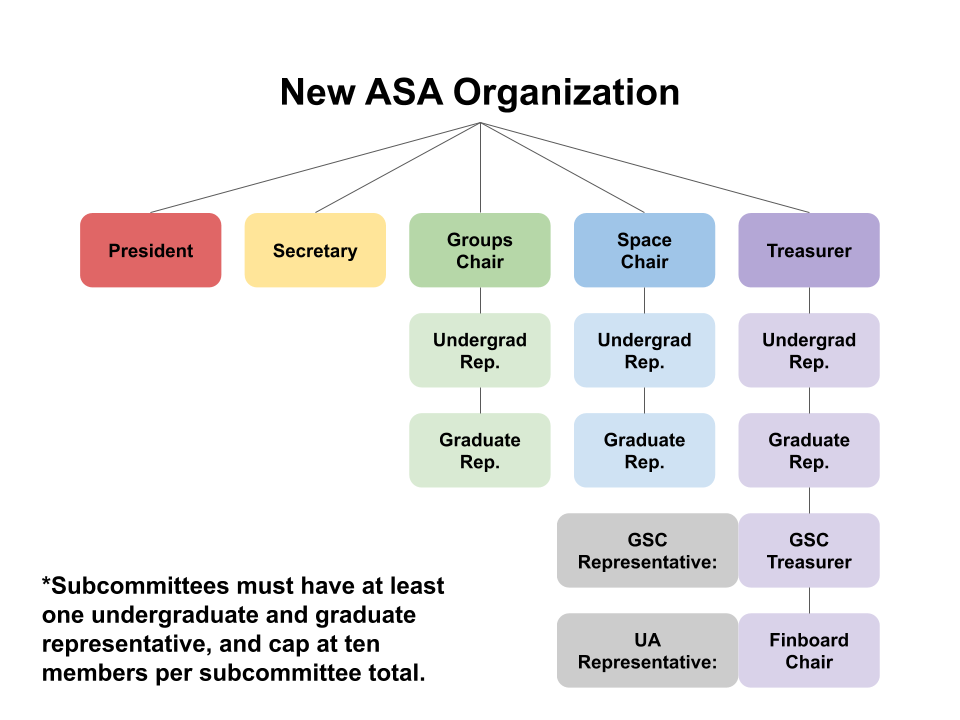
\includegraphics[width=1\linewidth]{asa_org_chart.png}
\end{figure}

\newpage

\appendix{ASA Recognition Procedures}
The ASA Recognition Procedures below are the formal guidelines for group recognition as called for by
the ASA Operating Guidelines.


\article{Applications}

\section{Timing}
Application deadlines will be set by the ASA Executive Board (herein referred to as "the Board") by
Registration Day of the given semester. Unless otherwise decided by a majority vote of the Board,
there will be one application deadline per semester.
\\

A group may apply for recognition no more than two times per school year, unless significant changes
have been made to the group’s purpose and/or structure or they receive advance permission from the
Board.
\\

Applications submitted in between deadlines will not be considered on a rolling basis and will only be
considered after the next deadline. Exceptions for extenuating circumstances can be requested by
contacting the Board. Applications submitted soon after a deadline may be considered with the
ongoing cycle of applications at the discretion of the Board.

\section{Requirements}
\begin{enumerate}[A.]
    \item \textit{Questions}: Application questions shall be set by the Board and may differ depending on the
classifications of groups as given in \hyperref[art:II_sect1]{Article II, Section 1}. Questions shall cover at least the
following topics:
    \begin{enumerate}[a.]
        \item Group purpose
        \item Uniqueness of group compared to existing recognized groups
        \item Size of group
        \item Needs for ASA recognition
        \item Classification requested – classifications are listed in \hyperref[art:II_sect1]{Article II, Section 1}. The Board
reserves the right to consider the application for classification(s) that are not requested,
however a group may decline recognition if they do not agree with a classification change.
    \end{enumerate}

    \item \textit{Membership}: A complete membership list shall be included. It must contain at least 5 MIT
students and be at least 50\% MIT students. More detailed guidelines for membership
requirements of an ASA-recognized group can be found in the ASA Operating Guidelines, \hyperref[art:I_sect3]{Article I, Section 3}.
Any group with fewer than 10 members at the time of their application will be
requested to submit a written plan to recruit and maintain members to assure the continuing
success and growth of their group.

    \item \textit{Constitution}: An application shall include a copy of the group’s constitution which must fulfill
all requirements set forth by ASA including but not limited to:
    \begin{enumerate}[a.]
        \item Group purpose
        \item Definition of membership including clauses reflecting:
        \begin{enumerate}[i.]
            \item Any member of the MIT community must be eligible for membership
            \item The organization shall not discriminate based on any characteristic listed in the
            \NDS for membership, officer position, or other
aspects.
        \end{enumerate}
    \item Definition of officer positions, which must include provisions for president and
treasurer (or corresponding officers). Those two positions shall be required to be
distinct MIT students.
    \item Procedures for officer elections and removal
    \item Procedure for member removal
    \item Clauses about meeting frequency, who presides over meetings, what meeting quorum is,
and how decisions can be made (ex: majority vote of active members present)
    \item Procedures for amending the constitution
    \item ASA Governance Clause:\\

The [activity name] agrees to abide by the rules and regulations of the Association of
Student Activities, and its executive board. This constitution, amendments to it, and the
by-laws of this organization shall be subject to review by the ASA Executive Board to insure
that they are in accordance with the aforementioned rules and regulations.
    \end{enumerate}
\end{enumerate}

\section{Meetings}
The Board may request a meeting with representatives of the group’s officers to discuss their
application or require that groups meet with other parties, such as MIT offices that can help the
Board make recognition decisions or with other groups about potential overlap of purpose. Such
meeting requirements will be conveyed to groups during the application process.


\article{Recognition Philosophy}

\section{Classifications}
Classifications for ASA-recognized student groups and their respective privileges can be found in the ASA
Operating Guidelines, \hyperref[art:I_sect2]{Article I, Section 2}.

\section{General Criteria}
\label{app:B_artII_sect2}
All groups shall be examined for the following criteria, at a minimum:
\begin{enumerate}
    \item \label{app:B_artII_sect2_1} At least 5 MIT students, at least 50\% MIT students.
    \item MIT student president and treasurer, or corresponding officers
    \item Follow \NDS and \MHL
    \item Legality – do not violate any Institute, local, state, or federal policies or laws
    \item Sustainability – potential for the group to last beyond the short term and the initial membership
    \item \label{app:B_artII_sect2_6} Appeal and scope of group purpose
    \item \label{app:B_artII_sect2_7} Uniqueness from existing groups, meaning: is the group unique or at all different from
existing groups?
\end{enumerate}
The Board will discuss new group applications for the criteria listed above with a representative
from the SOLE to ensure compliance with MIT policies. A group will be approved with a 2/3
majority vote of the ASA Board, during which the SOLE representative does not receive a vote.

\section{Funding Status Criteria}
Recognition overall shall be decided mainly on items \hyperref[app:B_artII_sect2_1]{1} through \hyperref[app:B_artII_sect2_7]{7} in the previous section. Items \hyperref[app:B_artII_sect2_6]{6} and
\hyperref[app:B_artII_sect2_7]{7} will be used to determine whether a group should be a Funded Student Group or an Unfunded
Student Group, as well as whether the group’s use of funds would follow GSC Funding Board and UA
FinBoard requirements. Funded Student Groups shall be those that demonstrate a broad scope,
potential for large appeal, significant distinction from existing groups, history of achievement, and a
demonstrated need for either GSC Funding Board or UA FinBoard funding.


\article{Completion of Recognition}
After the above requirements and criteria have been met and a group has been approved by a
majority vote of the Board, the group must complete the following requirements before their
recognition is official:
\begin{enumerate}
    \item Reply to recognition message sent by the Board with information on officer Kerberos IDs and
mailing lists
    \item Send the text of the \MHL to all group members
    \item Provide a current constitution that satisfies all ASA requirements
    \item Satisfaction and/or agreement to any conditions of the recognition decision
    \item Add members to student group page on Engage
\end{enumerate}
Groups shall have at least three weeks to submit the above materials. They shall also have at least three
weeks to complete any amendments to their constitution requested by the Board. These deadlines may
be set longer than prescribed and extensions may be granted at the discretion of the Board. If a group
does not meet the deadlines set forth and does not request an extension before the deadline, then
their application will be discarded and they will have to reapply for recognition.
\\

A group is only considered officially recognized when they have completed these steps and their group
has been added to the Engage by the Board.


\article{Appeals}
Recognition decisions may be appealed by email to the Board within two weeks of notification of the
decision. Said email shall include the basis for appeal and additional information the group deems
applicable and shall be no longer than 600 words, roughly one page.
\\

A meeting between the group and representatives of the Board may be requested by either party and
scheduled by the Board within two weeks of the request. Also at the request of either, a
representative of the Student Organizations, Leadership and Engagement Office may be asked to
attend the meeting.
\\

The Board may also request additional information, consultation meetings, support letters, or ask
more questions of the group before making a decision on the appeal. If the group does not respond
within two weeks, then the appeal shall be discarded.
\\

The original decision of the Board shall stand unless decided otherwise by a 2/3 vote of the Board. The
process for further appeals is outlined in the GSC and UA Bylaws


\article{Recognition of Derecognized Group}

\section{Applicability}
Re-recognition is possible for groups that have been previously recognized but were derecognized by the
Board for failure to complete the ASA re-recognition process or violation of ASA guidelines as soon as the
next semester after derecognition. The group shall apply following the standard group recognition
process and deadlines.

\section{Recognition Procedure}
A group of people that want to restart a group shall submit a new group application with all required
information as well as the following:
\begin{enumerate}
    \item A complete list of people involved with the restart effort – must include at least 5 MIT
students and be at least 50\% MIT students
    \item An account of any efforts made to contact the existing group’s officer list, listed officers,
and/or known past officers or members.
    \item Statement of purpose and plans for the activity
    \item Any plans to prevent the activity from going inactive or getting derecognized again
\end{enumerate}
The Board may request additional information or a meeting with group representatives. Then the
Board shall consider the request along with other new group applications. A majority vote of the
Board can decide to allow the requesting set of people to restart the activity. This decision can also
change the classification of an activity group (i.e. a Funded Student Group may be restarted as an
Unfunded Student Group).


\article{Classification Changes}
A group may request a classification change after one semester of recognition and no more than one
time per year.
\\

If a group wants to request a change from Unfunded Student Group status to Funded Student Group
status or from Sponsor-Funded Student Group status to a non-sponsored classification, then they shall
contact the Board with the information requested in the following \hyperref[app:B_artVI_sect1]{section}. Additional information or a
meeting with group representatives may be requested by the Board.
\\

For other classification changes a group should contact the Board about how to proceed.
\\

All classification changes require a majority vote of the Board to be approved.


\section{Unfunded Student Group to Funded Student Group}
\label{app:B_artVI_sect1}
Required information:
\begin{enumerate}
    \item Current and complete membership list
    \item The current purpose and scope of the group and how it has developed since the group’s
recognition or their previous request for a classification change
    \item Information about how Funded Student Group status would benefit the group and better
enable them to carry out their stated purpose
    \item How the group is unique and distinct from other groups (particularly Funded Student Groups)
\end{enumerate}
\,\hrule
\vspace*{1em}


\article{Re-Recognition}

\section{Annual Re-Recognition Procedure}
Once per year every ASA-recognized student group must complete the ASA re-recognition procedure.
Groups must complete these steps to maintain their recognized status:
\begin{enumerate}
    \item Five registered MIT student members must confirm their active membership in the group
    \item An officer of the group must affirm that the group abides by the \NDS
    \item An officer of the group must affirm that the group abides by the \MHL
\end{enumerate}
The ASA can also request further information such as updated group email lists, the number and
breakdown of members of the club, description of club activities, or other information deemed relevant
by the Board.
\\

There must be at least three weeks between the announcement of the re-recognition period and its
deadline. Club sports, FSILGs, and Dorms are not required to complete this process.

\section{Failure to Complete Re-Recognition Procedure}
Any group that does not complete the ASA re-recognition procedure after the deadline will have one
month to submit the required materials and maintain the group’s recognized status along with a fine for
late submission.
\\

Groups that do not complete the process after this extended period will be sent a derecognition notice
due to inactivity. A group that appeals after receiving a derecognition notice may be allowed to complete
the process but given the "Suspended" status for one academic year. "Suspended" groups have all the
rights of a non-suspended group, but will be immediately derecognized without appeal if the group does
not complete the re-recognition process on time during the next year’s cycle.

\article{Amendments}
This Operating Guidelines Appendix may only be modified via the process outlined in the GSC Bylaws %(\href{https://gsc.mit.edu/governing-documents/bylaws/#a2v}{Article II, Section G}, Subsection 5.iv.).
(\hyperref[bylaws:5iv]{Article II, Section G, Subsection 5.iv.}).

\newpage

\appendix{GSC Bylaws}
\label{app:C}

\setcounter{articlecount}{1}
\article{Committees}

\setcounter{sectioncount}{6}
\let\secnum\Alph
\let\subnum\Roman

\section{The following standing committees are established:}

The following shall be valid only if they are fully agreed upon by the MIT Graduate Student Council (GSC) and the MIT Undergraduate Association (UA), and included in the Bylaws of both groups. A majority vote of student group representatives during a General Body Meeting (as defined in Section v. below) shall be sufficient to force a vote of both the GSC and the UA Senate regarding a specific change to the following. Any references to the ASA Constitution shall refer to these Bylaws and the ASA operating guidelines (as defined below).

\subsection{Purpose}
The Association of Student Activities (ASA) shall be a joint committee of the MIT Graduate Student Council and the MIT Undergraduate Association (UA). Its purpose shall be to communicate the needs and interests of student groups to the GSC and UA, to promote student activities on the MIT campus, to serve the common interests of student activities, and to arbitrate conflicting interests.

\subsection{Executive Board}

The ASA shall consist of an Executive Board responsible for overseeing student activities on the MIT campus. This Board shall consist of at least the following members: president, treasurer, secretary, groups chair, and space chair. These members shall be elected at an ASA General Body Meeting, to be defined in Section v below. GSC and UA shall also each send one representative as an ex-officio member of the Executive Board. The ASA president shall have the same rights and responsibilities as chairs of other GSC and UA standing committees, with the exception of election and removal processes. All members must be registered MIT students and shall serve one-year terms.
\\

The Executive Board may also appoint additional members as necessary.

\subsection{Functions of the Executive Board}

The Executive Board shall recognize and derecognize student groups, maintain and distribute relevant information about all recognized groups, assign space to these groups, and arbitrate inter-activity disputes when requested by these groups to do so. The ASA shall interface with the MIT Student Organizations, Leadership, and Engagement Office as appropriate on all of these matters.

\subsection{Definition of Operating Guidelines}
\label{bylaws:5iv}

The ASA shall maintain a set of operating guidelines, to be made publicly available on its website, that explicitly define all relevant policies not included in these Bylaws regarding its roles and responsibilities. Specifically, these guidelines must outline responsibilities of the ASA Executive Board, procedures for the recognition and derecognition of student groups, rights and responsibilities of student groups with respect to the ASA, and guidelines that regulate the allocation and use of common student group resources (such as bulletin boards and office space). The ASA operating guidelines may be modified by a 2/3 vote of the entire ASA Executive Board. If either the GSC President and Treasurer or the UA President and Finance Board Chair oppose a given change, their veto must be sustained through the passing of legislation by either the GSC or the UA Senate, respectively. The GSC President and Treasurer, and UA President and Finance Board Chair must be informed of any changes to the ASA operating guidelines as soon as they are made. These changes must be communicated to all recognized student groups 24 to 48 hours after the GSC and UA have been informed, and shall go into effect 14 days after they are made. Changes to the ASA operating guidelines may be overturned by student groups either through a petition signed by the presidents or treasurers of 1/3 of these groups, or by a vote of the representatives of 1/3 of these groups taken at a General Body Meeting.

\subsection{General Body Meetings}

The ASA shall hold at least one General Body Meeting (GBM) per year, consisting of representatives from all recognized student groups. Quorum to proceed with a meeting shall be 30 or 20%, whichever is less, of these representatives, and all recognized student groups shall be informed of a GBM at least two weeks prior to the meeting. The presidents or treasurers of 1/3 recognized student groups may call a GBM through petition to the ASA Executive Board. The President, or ½ of the Executive Board, may also call a GBM. The GSC and UA Senate may also call a GBM through the passing of legislation.

\subsection{Oversight Mechanisms}

Any member of the ASA Executive Board, with the exception of the GSC and UA representatives, may be removed by a 2/3 vote of those attending a General Body Meeting. Executive Board members other than the President, Treasurer, GSC representative, and UA representative may also be removed by a ¾ vote of the Executive Board. Representatives appointed by the GSC and UA may be removed by their respective groups in the appropriate manner (as defined in the Constitutions or Bylaws of the GSC and UA, respectively). The ASA operating guidelines may specify additional mechanisms for officer removal.

\subsection{Appeals Process}

Student groups shall have the ability to appeal decisions made by the ASA at least once per semester. Appeals shall be heard by an Appeals Board consisting of the President and Treasurer of the GSC (or their proxies), the President and Finance Board Chair of the UA (or their proxies), and the President and one graduate and one undergraduate member of the ASA Executive Board. The ASA President shall be responsible for scheduling this appeals process. If an appeals process exists within the ASA Executive Board, student groups must follow that process before appealing to the GSC and UA. In addition, student groups may be requested to submit any relevant information to the Appeals Board, based upon which this Board may accept or reject their appeal without a meeting.
\end{document}

\end{document}